\epigraph{It is not new physics. It is the same physics --- just written down more honestly.}{}

\section{The Thought Experiment}


\begin{figure}[htbp]
\centering
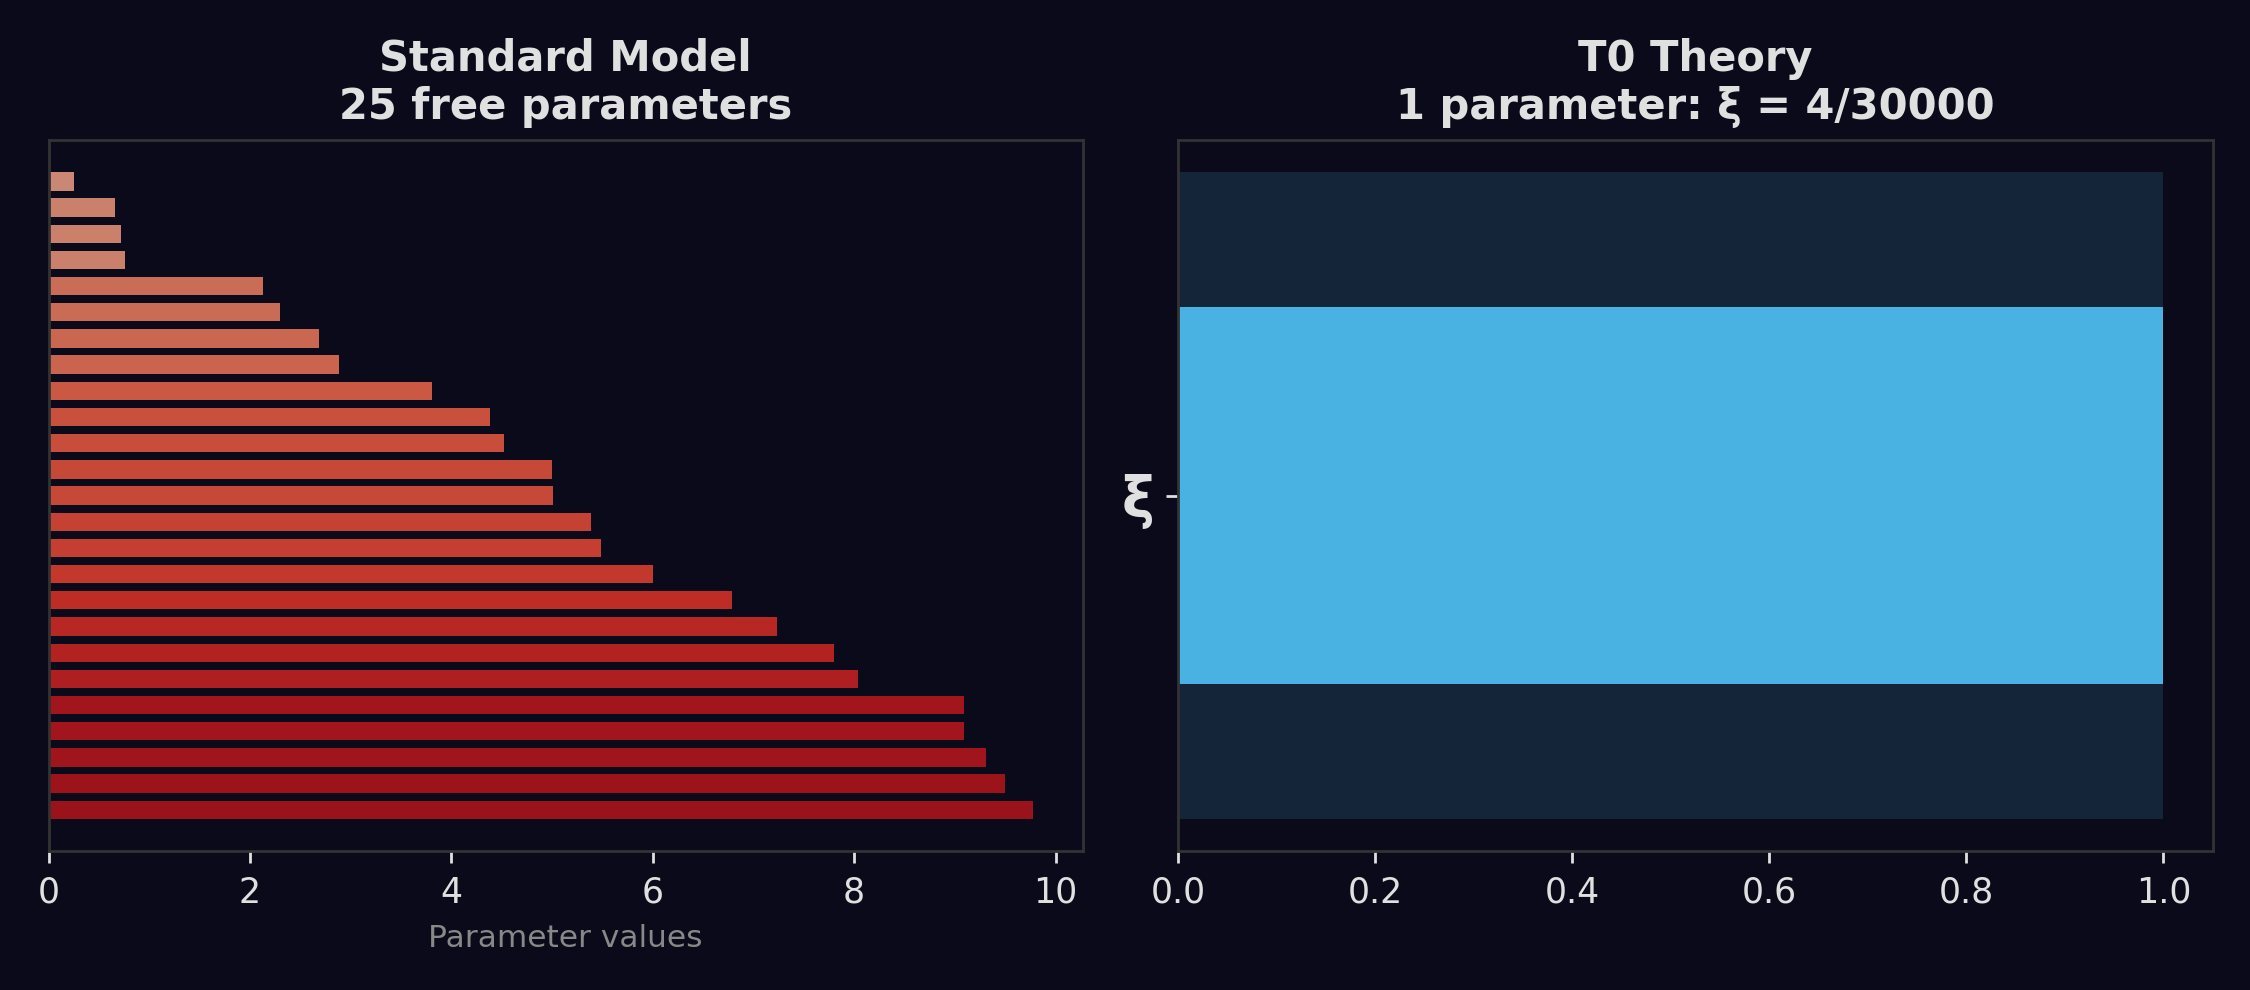
\includegraphics[width=0.85\textwidth]{img/ch02_comparison.png}
\caption{25~free parameters in the Standard Model vs.\ a single parameter~$\xi$ in T0.}
\end{figure}
Imagine sitting at an empty desk with permission to write down physics from scratch. No historical conventions, no evolved unit systems. Just the question: what is the simplest, most consistent system?

In particle physics it has been standard practice for decades to use natural units: $c = 1$ and $\hbar = 1$. Velocities are measured in fractions of the speed of light; energies and masses carry the same unit. This simplifies the equations considerably and reveals the underlying structure.

But there is one constant that is customarily \emph{not} set to one: the fine-structure constant~$\alpha \approx 1/137.036$. It describes the strength of the electromagnetic coupling and is regarded as a fundamental, dimensionless parameter of nature. Its value, according to the prevailing view, is a mystery --- a number we can measure but cannot explain.

\emph{What happens if we also set $\alpha = 1$?}

\section{Not a Contradiction but a Convention}

The first objection is obvious: $\alpha$ is dimensionless. Its value is $\approx 1/137$ in \emph{every} unit system. You cannot simply ``set it to one.''

But that is not quite right. What $\alpha = 1/137$ means depends on how we define the charge unit. In SI units $\alpha = e^2/(4\pi\varepsilon_0 \hbar c)$. In Gaussian units $\alpha = e^2/(\hbar c)$. The numerical value of $\alpha$ thus depends on the \emph{definition} of the elementary charge.

There are historical precedents:

\begin{itemize}
\item \textbf{George Johnstone Stoney}~(1874) defined the first system of natural units in which $e = 1$ was set --- implicitly introducing $\alpha$-dependent normalisations.
\item The \textbf{Heaviside-Lorentz system} rationalises Maxwell's equations through a redefinition of the charge unit that effectively achieves $\alpha = 1$.
\end{itemize}

Setting $\alpha = 1$ is therefore no physical contradiction. Concretely it means: one chooses the \emph{charge unit} so that the coupling constant appears as~$1$ in the equations. The physical content --- the fact that the electromagnetic coupling is weak ($\alpha_{\text{phys}} \approx 1/137$) --- does not vanish. It is absorbed into the geometry of~$\xsi$, just as with $c = 1$ the difference between metres and seconds is absorbed into conversion factors.

What changes are numerical values. What does \emph{not} change are all physical predictions, all experiments, all measurable ratios.

\begin{kerngedanke}
$\alpha = 1$ is not new physics. It is a redefinition of the charge unit that radically simplifies the unit system. The physical information $\alpha_{\text{phys}} \approx 1/137$ is preserved --- it now resides in~$\xsi$. Just as $c = 1$ does not mean light is slow, $\alpha = 1$ does not mean the electromagnetic coupling is strong.
\end{kerngedanke}

\section{$\alpha$ as the Fundamental Input}

Here comes the decisive turn. If we work in a system where $c = \hbar = \alpha = 1$, then we need exactly \emph{one} measured value to establish the connection to physical reality: the experimental value $\alpha \approx 1/137.036$.

From $\alpha$ a geometric parameter can be derived:
\begin{equation}
\xsi = \frac{\alpha}{(E_0/1\,\text{MeV})^2} = \frac{4}{3} \times 10^{-4}
\end{equation}
where $E_0 = \sqrt{m_e \cdot m_\mu} = 7.398$~MeV is the characteristic energy scale, defined by the geometric mean of the electron and muon masses.

From $\xsi$ follows \emph{everything}:
\begin{itemize}
\item All particle masses --- via $\xsi$-quantisation
\item The gravitational constant --- $G = \xsi^2/(4m_e)$ times conversion factors
\item The Planck length --- $\lP = \xsi/(2\sqrt{m_e})$
\item The speed of light --- geometrically determined by $\xsi$
\item The Boltzmann constant --- a pure unit convention
\end{itemize}

\begin{zusammenfassung}
\textbf{One measurement. Nothing else. Everything else is geometry.}

The whole of physics --- from particle masses through gravitation to cosmology --- reconstructs itself from a single measured parameter, the fine-structure constant $\alpha$, and the geometric constant $\xsi = \frac{4}{3} \times 10^{-4}$.
\end{zusammenfassung}

\section{The Derivation Chain}

The logic unfolds as a cascade:

\begin{center}
\begin{tikzpicture}[
  box/.style={draw, rounded corners, minimum width=3cm, minimum height=0.8cm, text centered, fill=blue!8},
  arr/.style={-{Stealth[length=3mm]}, thick}
]
\node[box] (alpha) at (0,0) {$\alpha$ (measured)};
\node[box] (xi) at (0,-1.5) {$\xsi$ (geometric)};
\node[box] (masses) at (-3,-3) {Particle masses};
\node[box] (G) at (0,-3) {$G$ (gravitation)};
\node[box] (lp) at (3,-3) {$\lP$ (Planck)};
\node[box] (c) at (0,-4.5) {$c$ (speed of light)};
\node[box] (L0) at (3,-4.5) {$L_0 = \xsi \cdot \lP$};

\draw[arr] (alpha) -- (xi);
\draw[arr] (xi) -- (masses);
\draw[arr] (xi) -- (G);
\draw[arr] (xi) -- (lp);
\draw[arr] (G) -- (c);
\draw[arr] (lp) -- (L0);
\end{tikzpicture}
\end{center}

In T0 natural units: $c = \hbar = \alpha = G = 1$. The SI values are recoverable at any time --- they are merely conversion factors, not fundamental quantities.

And here the circle closes back to the SI reform: the reform of~2019 \emph{unwittingly} implemented precisely the calibration that is consistent with the $\xsi$-geometry. It was the first step on a path that the T0 theory follows to its end.
